\PassOptionsToPackage{unicode=true}{hyperref} % options for packages loaded elsewhere
\PassOptionsToPackage{hyphens}{url}
%
\documentclass[english,pdf]{apa6}
\usepackage{lmodern}
\usepackage{amssymb,amsmath}
\usepackage{ifxetex,ifluatex}
\usepackage{fixltx2e} % provides \textsubscript
\ifnum 0\ifxetex 1\fi\ifluatex 1\fi=0 % if pdftex
  \usepackage[T1]{fontenc}
  \usepackage[utf8]{inputenc}
  \usepackage{textcomp} % provides euro and other symbols
\else % if luatex or xelatex
  \usepackage{unicode-math}
  \defaultfontfeatures{Ligatures=TeX,Scale=MatchLowercase}
\fi
% use upquote if available, for straight quotes in verbatim environments
\IfFileExists{upquote.sty}{\usepackage{upquote}}{}
% use microtype if available
\IfFileExists{microtype.sty}{%
\usepackage[]{microtype}
\UseMicrotypeSet[protrusion]{basicmath} % disable protrusion for tt fonts
}{}
\IfFileExists{parskip.sty}{%
\usepackage{parskip}
}{% else
\setlength{\parindent}{0pt}
\setlength{\parskip}{6pt plus 2pt minus 1pt}
}
\usepackage{hyperref}
\hypersetup{
            pdftitle={Sans Forgetica is Really Forgettable},
            pdfkeywords={Disfluency, Recall, Desirable Difficulty, Learning and Memory},
            pdfborder={0 0 0},
            breaklinks=true}
\urlstyle{same}  % don't use monospace font for urls
\usepackage{graphicx,grffile}
\makeatletter
\def\maxwidth{\ifdim\Gin@nat@width>\linewidth\linewidth\else\Gin@nat@width\fi}
\def\maxheight{\ifdim\Gin@nat@height>\textheight\textheight\else\Gin@nat@height\fi}
\makeatother
% Scale images if necessary, so that they will not overflow the page
% margins by default, and it is still possible to overwrite the defaults
% using explicit options in \includegraphics[width, height, ...]{}
\setkeys{Gin}{width=\maxwidth,height=\maxheight,keepaspectratio}
\setlength{\emergencystretch}{3em}  % prevent overfull lines
\providecommand{\tightlist}{%
  \setlength{\itemsep}{0pt}\setlength{\parskip}{0pt}}
\setcounter{secnumdepth}{0}

% set default figure placement to htbp
\makeatletter
\def\fps@figure{htbp}
\makeatother

% Manuscript styling
\usepackage{upgreek}
\captionsetup{font=singlespacing,justification=justified}

% Table formatting
\usepackage{longtable}
\usepackage{lscape}
% \usepackage[counterclockwise]{rotating}   % Landscape page setup for large tables
\usepackage{multirow}		% Table styling
\usepackage{tabularx}		% Control Column width
\usepackage[flushleft]{threeparttable}	% Allows for three part tables with a specified notes section
\usepackage{threeparttablex}            % Lets threeparttable work with longtable

% Create new environments so endfloat can handle them
% \newenvironment{ltable}
%   {\begin{landscape}\begin{center}\begin{threeparttable}}
%   {\end{threeparttable}\end{center}\end{landscape}}
\newenvironment{lltable}{\begin{landscape}\begin{center}\begin{ThreePartTable}}{\end{ThreePartTable}\end{center}\end{landscape}}

% Enables adjusting longtable caption width to table width
% Solution found at http://golatex.de/longtable-mit-caption-so-breit-wie-die-tabelle-t15767.html
\makeatletter
\newcommand\LastLTentrywidth{1em}
\newlength\longtablewidth
\setlength{\longtablewidth}{1in}
\newcommand{\getlongtablewidth}{\begingroup \ifcsname LT@\roman{LT@tables}\endcsname \global\longtablewidth=0pt \renewcommand{\LT@entry}[2]{\global\advance\longtablewidth by ##2\relax\gdef\LastLTentrywidth{##2}}\@nameuse{LT@\roman{LT@tables}} \fi \endgroup}

% \setlength{\parindent}{0.5in}
% \setlength{\parskip}{0pt plus 0pt minus 0pt}

% \usepackage{etoolbox}
\makeatletter
\patchcmd{\HyOrg@maketitle}
  {\section{\normalfont\normalsize\abstractname}}
  {\section*{\normalfont\normalsize\abstractname}}
  {}{\typeout{Failed to patch abstract.}}
\makeatother
\shorttitle{Sans Forgetica}
\author{Jason Geller\textsuperscript{1}, Sara D. Davis\textsuperscript{2}, \& Daniel Peterson\textsuperscript{2}}
\affiliation{
\vspace{0.5cm}
\textsuperscript{1} University of Iowa\\\textsuperscript{2} Skidmore College}
\authornote{Jason Geller, Department of Psychology and Brain Sciences, University of Iowa, W113 Seashore Hall, Iowa City, IA, 52242; Department of Psychology, University of Missouri, Columbia, MO, 65211; Nathan Nunley, University of Mississippi, P.O. Box 1848, University, MS, 28677.


Correspondence concerning this article should be addressed to Jason Geller, Department of Psychological and Brain Science, W113 Seashore Hall, Iowa City, IA, 52242. E-mail: jason-geller@uiowa.edu}
\keywords{Disfluency, Recall, Desirable Difficulty, Learning and Memory\newline\indent Word count: 4257}
\usepackage{lineno}

\linenumbers
\usepackage{csquotes}
\usepackage{endnotes}
\let\footnote\endnote
\ifnum 0\ifxetex 1\fi\ifluatex 1\fi=0 % if pdftex
  \usepackage[shorthands=off,main=english]{babel}
\else
  % load polyglossia as late as possible as it *could* call bidi if RTL lang (e.g. Hebrew or Arabic)
  \usepackage{polyglossia}
  \setmainlanguage[]{english}
\fi

\title{Sans Forgetica is Really Forgettable}

\date{}

\abstract{
Do students learn better with material that is perceptually harder-to-process? While evidence is equivocal on the matter, recent claims suggest that placing materials in Sans Forgetica font, which is perceptually hard-to-process, has positive effects on student learning. Given the weak evidence for perceptual disfluency effects, this led us to examine the mnnmonic effects of Sans Forgetica more closely. In two preregistered experiments, we tested if Sans Forgetica is really unforgetable. In Experiment 1 (\emph{N} = 233), participants studied weakly realted cue-target pairs with targets presented in either Sans Forgetcia or with missing letters (e.g., G\_RL). Cued recall performance showed a robust generation effect, but no Sans Forgetica memory benefit. In Experiment 2 (\emph{N}=528), participants read a passage about ground water with select sentences presented in either Sans Forgetcia, yellow highlighting, or unmodified. Cued recall for select words were better for pre-highlighted information than when unmodified. Critically, presenting sentences in Sans Forgetica did not produce better cued recall than pre-highlighted sentences or sentences presented unchanged. Our findings suggest that Sans Forgetica is really forgeticable.
}

\begin{document}
\maketitle

Students want to remember more and forget less. Being able to recall and apply previously learned information is key for successful learning. Decades of research in the laborartory and in the classroom have put forth the paradoxical idea that making learning harder (not easier) should have the desirable effect of improving long-term retention of material--called the desirable difficulty principle (Bjork \& Bjork, 2011). Notable examples of desirable difficulties include having participants generate information from word fragments instead of passively reading intact words (Bertsch, Pesta, Wiscott, \& McDaniel, 2007), spacing out study sessions instead of massing them (Carpenter, 2016), and having participants engage in retrieval practice after studying instead of simply restudying the information (Kornell \& Vaughn, 2016). Another simple strategy that has gained some attention is to make material more perceptually disfluent. This can be done by changing the material's perceptual characteristics. Visual material that is masked (Mulligan, 1996), inverted (Sungkhasettee, Friedman, \& Castel, 2011), presented in an atypical font (Diemand-Yauman, Oppenheimer, \& Vaughan, 2011; French et al., 2013), blurred (Rosner, Davis, \& Milliken, 2015), or even in handwritten cursive (Geller, Still, Dark, \& Carpenter, 2018) have all been shown to produce memory benefits. The desirable effect of perceptual disfluency on memory is called the disfluency effect (Bjork \& Yue, 2016).

Although appealing as a pedagogical strategy due to the relative ease of implementation, there have been several experiments that failed to find memorial benefits for perceptually disfluent materials {[}e.g., Magreehan, Serra, Schwartz, and Narciss (2016); Rhodes and Castel (2008), Rhodes and Castel (2009); Rummer, Schweppe, and Schwede (2016); Yue et al. (n.d.)), casting doubt upon the robustness of the disfluency effect. Corrobroating this, A recent meta-analysis by Xie, Zhou, and Liu (2018) with 25 studies and 3,135 participants found a small, nonsignificant, effect of perceptual disfluency on recall and (\emph{d} = -0.01) and transfer (\emph{d} = 0.03). Despite having no mnnmemonic effect, perceptual disfluency produced longer reading times (\emph{d} = 0.52) and lower judgments of learning (\emph{d} = -0.043). In the laboratroy, Geller et al. (2018) and Geller \& Still (2018) manpiulated several boundary conditions (e.g., level of degradation, type of judgement of learning, retentional interval, and testing expectany) and found you can get positive memory effects from perceptual disflunet mateirals (in recognition), but it is not robust. Taken together, the evidence is weak for perceptual disfluency being a desriable difficulty.

Despite the weak evidence, perceptual disfluency is still being touted as a viable learning tool, especially in the popular press. Recently, reputable news sources like the Washington Post (\url{https://www.washingtonpost.com/business/2018/10/05/introducing-sans-forgetica-font-designed-boost-your-memory/}) and National Public Radio (NPR; \url{https://www.npr.org/2018/10/06/655121384/sans-forgetica-a-font-to-remember}) claimed that a new font called Sans Forgetica could enhance memory, despite only unplublished evidence being available at the time (Earp, 2018). It is thought that the mnnemonic benefit is due to the characteristics of the font. Sans Forgteica is a variation of a sans-serif typeface that consists of intermitten gaps in letters that are back slanted (see fig. 1). Since the release of those news articles, the Sans Forgetica font is available on all operating systems (download the font file), some browsers (e.g., Chrome), and can be downloaded on your phone.

\begin{figure}
\includegraphics[width=2.36in]{/Users/hang/SF_Expt2/SF} \caption{Example of Sans Forgetica font. }\label{fig:unnamed-chunk-1}
\end{figure}

\hypertarget{current-studies}{%
\subsection{Current Studies}\label{current-studies}}

Given the weak evidence for the disfluency effect, we thought it pertinent to empircally examine whether Sans Forgetica produces more durabale learning. The question of whether Sans Forgetica produces a mnnmenomic benefits has clear practical implications. In the educational domian, it would be relatively quick and easy to use Sans Forgetica. However, in order for the Sans Forgetica to be useful, it is importnat to note and understand both its successes and failures. To the authors' knowledge, there is only one peer-reviewed paper (Eskenazi \& Nix, 2020) examining the effectivenss of Sans Forgetica in generating a desirable difficlty. In one experiment Eskenazi and Nix (2020) found that words and definitions in Sans Forgetica font lead to better orthographic discriminabity and semantic acquisition, but only if participnats were good spellers. From this one study, it is not clear if the benefits of Sans Forgetica font extends to other memory processes, as the Eskenazi and Nix (2020) study focused on lexical acquistion (orthographic and semantic features of a word). Given this, we felt it was pertinent to examine the effectiveness of Sans Forgetica in two different memory expeirments. To this end,we conducted to two high-powered preregistered experiments examining whether (1) recall is better in Sans Forgetica font and (2) how it compares with other notable learning techniques--generation (Experiment 1) and pre-highlighting (Experiment 2). Comparing Sans Forgetica to other study techniques allows us to examine the mechanisms underlying the effect, if any.

\hypertarget{experiment-1}{%
\section{Experiment 1}\label{experiment-1}}

In Experiment 1 we were interested in answering two questions. First, is Sans Forgetica more memorable than a normal, fluent, font (e.g., Arial)? Second, is the Sans Forgetica effect on memory similar in magnitude to the generation effect? While very is known about Sans Forgetica, one of the most intuitively appealing theories for why Sans Forgetica font benefits memory is that of mental effort. It is believed that reading materials in Sans Forgetica requires more effort than simply reading a normal font. Essentailly, the intermiten gaps of Sans Forgetica requires readers to generate or fill in the missing pieces producing a memory advantage. This mechanism of action is simiar to that of the generation effect, wherein information is better remembered when generated or filled-in compared to if it is simply read. In Experiment 1 we examined the mnnemonic benefit of Sans Forgetica and generation by looking at cued recall performance with weakly realted pairs. If Sans Forgetica does produce a mnnmoneic benefit, we should observe better cued recall performance for targets in Sans forgetica font comarped to Arial font. Futhrer, if it is similar to the generation effect, the magnitude of the memory benefit between the two should be similar.

\hypertarget{method}{%
\subsection{Method}\label{method}}

\hypertarget{participants}{%
\subsubsection{Participants}\label{participants}}

Two-hundred and thirty people from Amazon's Mechanical Turk Service participated for money. Sample size was based on a priori power analyses conducted using PANGEA v0.2 (Westfall, 2015). Sample size was calculated based on the smallest effect of interest (SEOI; Lakens \& Evers, 2014). In this case, we were interested in powering our study to detect medium-to-large effect size (\emph{d} = .35). We choose this effect size as our SESOI due in part to the small effect sizes seen in actaul classroom studies (Bulter et al., 2014). Therefore, assuming an alpha of .05 and a desired power of 90\%, a sample size of 230 is required to detect whether an effect size of .35 differs from zero. After excluding participants who 1) did not complete every phase of the experiment, 2) started the experiment multiple times, 3) reported experiencing technical problems did not indicate that they were fluent in English {[}\^{}2{]}: This question was not asked during the experiment., or 5) reported seeing our stimuli before, we were left with 115 participants per group.

\hypertarget{materials}{%
\subsubsection{Materials}\label{materials}}

The preregistration for Experiment 1 can be found here: \url{https://aspredicted.org/3ai98.pdf}. All materials, data, and analysis scirpts for both Experiment 1 can be found here (\url{https://osf.io/d2vy8/}). The results contained herein are computationally reproducible by going to the primary author's github repository for the paper (\url{https://github.com/jgeller112/SF_Expt2}) and clicking on the binder button.

Participants were presented with 22 weakly related cue-target pairs taken from Carpenter, Pashler, and Vul (2006)){[}\^{}1{]}: Two cue-target pairs (e.g., range-rifle and train-plane) had to be thrown out as they were not preseted due to a coding error. The cue-target pairs were all nouns, 5--7 letters and 1--3 syllables in length, and high in concreteness (400--700) and frequency (at least 30 per million). Free association norms (Nelson, McEvoy, \& Schreiber, 2004) were used to create 22 weakly associated pairs of similar forward and backward strength. Two counterbalanced lists were created for each difficulty type group(generation and Sans Forgetica) so that each item could be presented in each disfluency conditions without repeating any items for an individual participant.

\hypertarget{design-and-procedure}{%
\subsubsection{Design and Procedure}\label{design-and-procedure}}

Disfluency (fluent vs.~disfluent) was manipulated within-subejcts and within-items and difficulty type (Generation vs.~Sans Forgetcia) was manipulated between participants. For half the participants, targets were presented in Sans Forgetica while the other half were presented in Arial font; for the other half of participants, targets were presented with missing letters (vowels were replaced by underscores) and the other half were intact (Arial font). After a short 2 minute distractor task (anagram generation), they completed a cued recall test. During cued recall, particpants were presented 24 cues one at a time and asked to provide the target word. After they were thanked and debriefed.

Particpants completed the experiment on-line via the Qualtrics survey platfom hosted on Amazon Mechainal Turk. After reading and consenting, participants were randomly assigned to one of two conditions: The generation condition or the Sans Forgetica condition. Participants were told to study word pairs so that later they could recall second word (target) when cued with the first word (cue). The experiment began with the presentation of 22 word pairs, shown one at a time, for 2 secconds each. The cue word always appeared on the left and the target always on the right. Immediately proceeding this, participants did a short 2 minute distractor task (anagram generation). Finally participants completed a cued recall test. During cued recall, particpants were presented 22 cues one at a time and asked to provide the target word. Responses were self-paced. Once completed, participants clicked on a button to advance to the next question. At the end, participants were asked several demographic questions.

\hypertarget{scoring}{%
\subsubsection{Scoring}\label{scoring}}

Spell checking was automated with the hunspell package in R (Ooms, 2018) using spellCheck.R. A nice walkthrough on how to use the package can be found in Buchanan, De Deyne, and Montefinese (2019). Using the package, each response was corrected for misspelings. Corrected spellings are provided in the most probable order, therefore, the first suggestion is selected as the correct answer. As a second pass, we manually examined the output to catch incorrect suggestions and to add their own correction. If the response was close to the correct response, it was marked as correct. Becasuse participants were recruited in the United States, we used the American English dictionary.

\hypertarget{results-and-discussion}{%
\section{Results and Discussion}\label{results-and-discussion}}

Although we had pre-registered a simple 2 X 2 mixed ANOVA approcah, we opted for a more powerful analytic approach that better represents the data: generalized linear mixed modeling. Models were fit in R (vers. 3.5.0; R Core Team, 2019) with the lme4 package (vers. 2.3.1; Bates, Mächler, Bolker, \& Walker, 2015). All models were analyzed using maximal random effects structures with random slopes where allowed ({\textbf{???}}). All figures were created with ggplot (Wickham, 2016). We fit a logistic mixed model to predict cued recall accuracy with difficulty type (generation vs.~sans forgetcia) and disfluency (fluent vs.~disfluency). We fit the maximal model (formula: \enquote{glmer(acc\textasciitilde{}difftypedisflu + (1+disflu\textbar{}ResponseID) + (1+difftype\textbar{}target), family=binomial, data=data}). Effect sizes (Cohen's \emph{d}) were labelled following ({\textbf{???}}) recommendations. The effect of difficulty type was nonsignificant, \emph{b} = -0.09, \emph{SE} = 0.11, 95\% CI {[}-0.30, 0.13{]}, std. beta = -0.09, \emph{p} = 0.431, \emph{d} = 0.05). Individuals did recall more disfluent target words than fluney target words, \emph{b} = 0.21, \emph{SE} = 0.06, 95\% CI {[}0.09, 0.33{]}, std. beta = 0.22, p \textless{} .001, \emph{d} = 0.12). This was qualifed by an interaction between difficulty type and disfluency was significant, \emph{b} = 0.22, \emph{SE} = 0.04, 95\% CI {[}0.14, 0.30{]}, std. beta = 0.21, \emph{p} \textless{} .001, \emph{d} = .11). A Bayes factor was derived using the brms package {[}Bürkner (2018); vers. 2.3.1{]} to determine the strength of the interaction effect. We used normal priors on all fixed effects. These are uninformative in terms of direction--both positive and negative effects are equally likely--but they are informative in terms of magnitude. The prior indicated that a model with the interaction term was strongly preferred over the model without the interaction {[}BF \textgreater{} 100; (``Jeffreys, H. (1961) Theory of Probability. 3rd Edition, Clarendon Press, Oxford. - References - Scientific Research Publishing,'' n.d.)). This suggests that the magnitide of the generation effect is larger than the magnitude of the Sans Forgetica effect. This can be clearly seen in Fig. 2.

\begin{verbatim}
## Warning: Missing column names filled in: 'X1' [1]
\end{verbatim}

\textbackslash{}begin\{figure\}

\{\centering 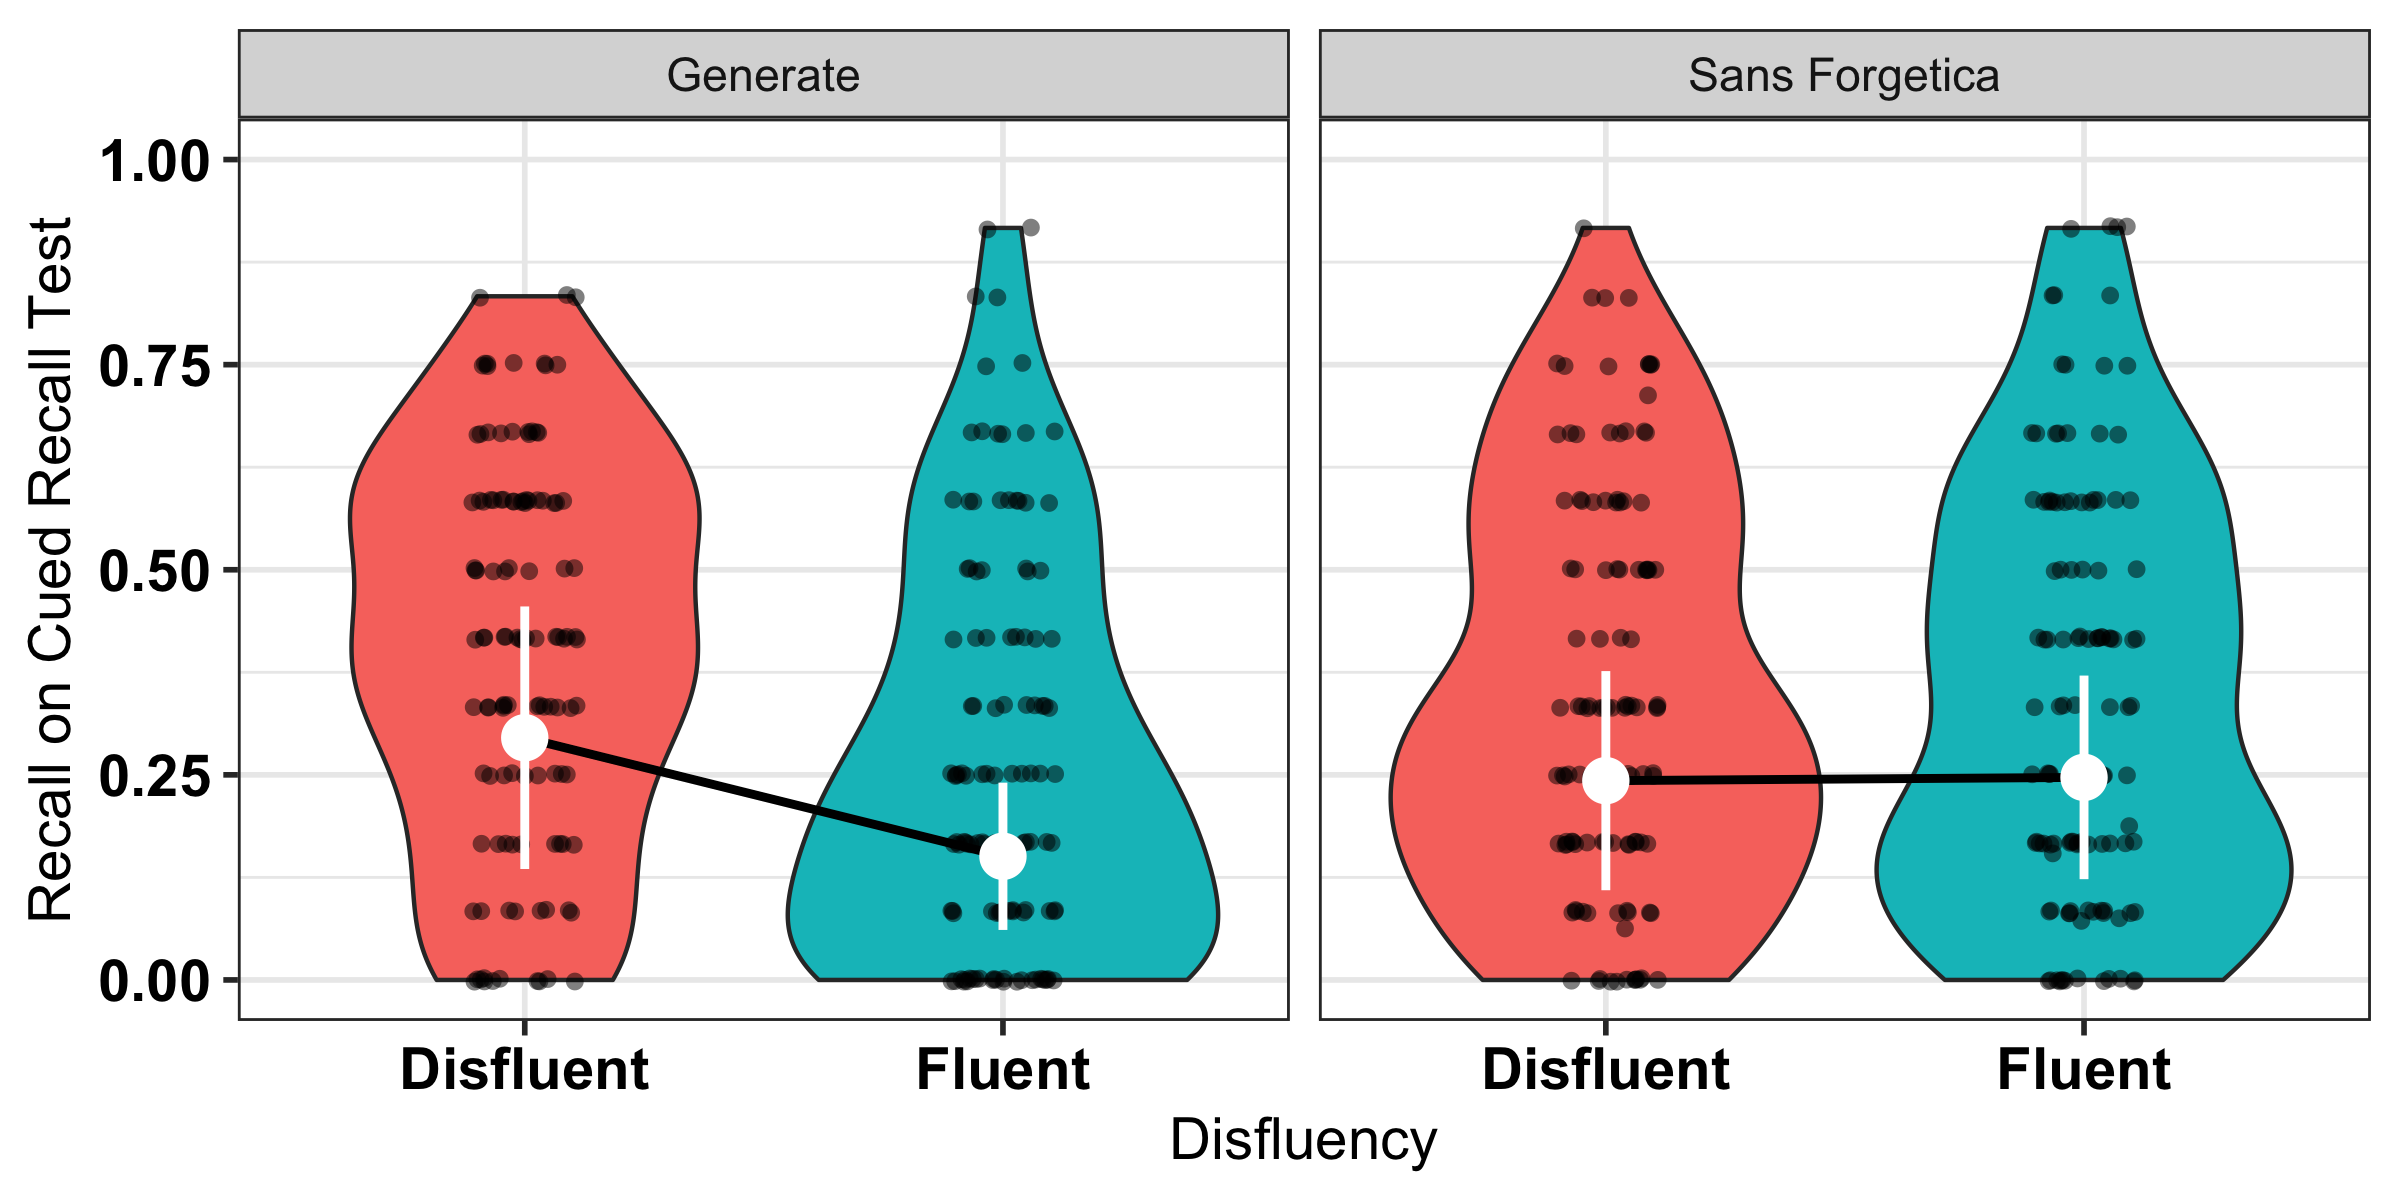
\includegraphics{SF_Paper_files/figure-latex/unnamed-chunk-2-1}

\}

\textbackslash{}caption\{Accuracy on Cued Recall Test. 95\% CIs dervied from the glmer model using the effects package in R.\}\label{fig:unnamed-chunk-2}
\textbackslash{}end\{figure\}

The results for Experiment 1 are clear-cut. Cued recall for items presented intact and in Sans Forgetica font were equivocial. That is, we did not observe a memory benefit for Sans Forgetica font. We did, however, observe greater recall for generated items, which replicates decades of litearture (Bertsch et al., 2007). This suggests that (1) presenting materials in Sans Forgetica does not lead to better memory and (2) the Sans Forgetica effect is most likely not a desirable difficulty.

\hypertarget{experiment-2}{%
\section{Experiment 2}\label{experiment-2}}

Experiment 1 failed to find a memory benefit for Sans Forgetica effect. A limitation of Experiment 1 is that simple stimulus-response learning lacks educational realsim. To remedy this, Experiment 2 tested the mnemonic effects of Sans Forgetica using more realistic materials. Whereas Experiment 1 tested whether Sans Forgetica is driven by the generative process of retreival, Experiment 2 examined whether the Sans Forgetcia effect might exert its mnnmenonic benefit by making material more distinctive. Specifically, Sans Forgetica may make the marked portion of text more memorable because it stands out from the surrounding text. This is similar to the effects of pre-highlighting on learning. Indeed, some evidence supports this type of role for highlighting: When students read pre-highlighted passages, they recall more of the highlighted information and less of the non-highlighted information compared to students who receive an unmarked copy of the same passage (Fowler \& Barker, 1974; Silvers \& Kreiner, 1997). To this end, Experiment 2 compared cued recall performance on a passage where some of the sentences were either presented in: Sans Forgetica, pre-highlighted in yellow, or unmodified. We hypothesized that if the Sans Forgetica effect is mainly driven by distinctiveness, words presented in Sans Forgetica should benefit more from the disfluency than the passage presented unmodified. Further, the benefit for Sans Forgetica should be similar in magnitude to the pre-highlighting condition as both manipulations serve to increase the distinctivness of the text.

The pre-registration form for Experiment 2, which includes hypotheses, planned analyses,exclusion criteria, and sample size justification, can be found at: \url{https://aspredicted.org/3jz3z.pdf}.

\hypertarget{method-1}{%
\subsection{Method}\label{method-1}}

\hypertarget{participants-1}{%
\subsubsection{Participants}\label{participants-1}}

Five hundred and twenty-eight undergraduates participated for partial completion of course credit. Sample size was based on a priori power analyses conducted using PANGEA v0.2. Sample size was calculated based on the samllest effect of interest (Lakens \& Evers, 2014). Similar to Experiment 1, we were interested in powering our study to detect a medium-sized effect size (\emph{d} = .35). Therefore, assuming an alpha of .05 and a desired power of 90\%, a sample size of 170 per group is required to detect whether an effect size of .35 differs from zero. After excluding participants based on our preregistered exclusion critera, we were left with unequal group sizes. Becasue of this, we ran six more pariticpants per group, giving us 176 participants in each of the three conditions.

\hypertarget{materials-1}{%
\subsubsection{Materials}\label{materials-1}}

Participants read a passage on ground water (856 words) taken from from the U.S. Geological Survey (see {\textbf{???}}). Eleven critical phrases\footnote{orginally we had 12 critical phrases but a pilot test showed that one of the questions was repeated twice so we removed one of them and also added a manipulation check question to sure participants were paying attention} each containing a different keyword, were selected from the passage (e.g., the term \emph{recharge} was the keyword in the phrase: Water seeping down from the land surface adds to the ground water and is called recharge water.) and were either presented in SF, highlighted, or unmodified. Then, 11 fill-in-the blank questions were created from these phrases by deleting the keyword and asking participants to provide it on the final test (e.g., Water seeping down from the land surface adds to the ground water and is called \_\_\_\_\_\_\_\_\_\_ water). There was 1 manipulation check question: \enquote{What was the passage you read on?.}

\hypertarget{design-and-procedure-1}{%
\subsubsection{Design and Procedure}\label{design-and-procedure-1}}

Participants were randomly assigned to either the pre-highlighted condition, sans forgetica condition, or unmodified condition. Our design manipulated three difference types of passages between-subjects: pre-highlighting, Sans Forgetica, and unmodified.

Participants completed the experiment on-line via the Qualtrics survey platform. After reading and signing a consent form, participants were randomly assigned to one of three conditions: pre-highlighing, Sans Forgetica, or unmodified. Participants read a passage on ground water. All particiapnts were instructed to read the passage as though they were studying material for a class. After 10 minutes, all participants were given a brief questionnaire (2 questions) asking them to indicate their metacognitive beliefs afte reading the passage. The two questions were: \enquote{Do you feel that the presentation fo the material helped you remember} and \enquote{How likely is it that you will be able to recall material from the passage you just read on a scale of 0 (not likely to recall) to 100 (likely to recall) in 5 minutes?} Participants were then given a short distractor task (anagrams) for 3 minutes. Finally, all participants were given 12 fill-in-the-blank test questions, presented one at a time.

\hypertarget{scoring-1}{%
\subsubsection{Scoring}\label{scoring-1}}

Spell checking was automated with the same procedure as Experiment 1.

\hypertarget{results-and-discussion-1}{%
\subsection{Results and Discussion}\label{results-and-discussion-1}}

For congruency with Experiment 1, we fit a logistic mixed model in a similar fashion (this goes against our pre-registration). We fit a model with passage type as a fixed effect and random intercepts for participants (\emph{N}=528) and questions (\emph{N}=11): (formula: acc=glmer(auto\_acc\textasciitilde{}passage\_type+(1\textbar{}Participant) + (1\textbar{}Question), data=data, family=\enquote{binomial}). Passage type was coded using treatment coding. We hypothesized that recall for pre-highlighted and Sans Forgetica sentences would be better remembered than normal sentences and that there would be no recall differences between the highlighted and sans forgetia sentences. Our hypotheses were partially supported (see Fig. 2). Results indicated that pre-highlighted sentences were better remembered than sentences presented normally, \emph{b} = 0.38, \emph{SE} = 0.17, 95\% CI {[}0.05, 0.71{]}, std. beta = 0.38, \emph{p} \textless{} .05, \emph{d} = 0.21, and were marginally better remembered than sentences presented in Sans Forgetcia, \emph{b} = -.317, \emph{exp(B)} = 1.37, \emph{SE} = .168, \emph{z} = -1.89, \emph{p} = .059, \emph{d} = -0.18. Critically, there was no difference between sentences presented normally and in Sans Forgetcia, \emph{b}= 0.06, \emph{SE} = 0.17, 95\% CI {[}-0.26, 0.39{]}, std. beta = 0.06, \emph{p} = 0.700, \emph{d} = .03. A Bayes factor using the brms package {[}Bürkner (2018)) was computed and there is moderate evidence that there is no difference between the two conditions (BF01 = 7.47).

\textbackslash{}begin\{figure\}

\{\centering 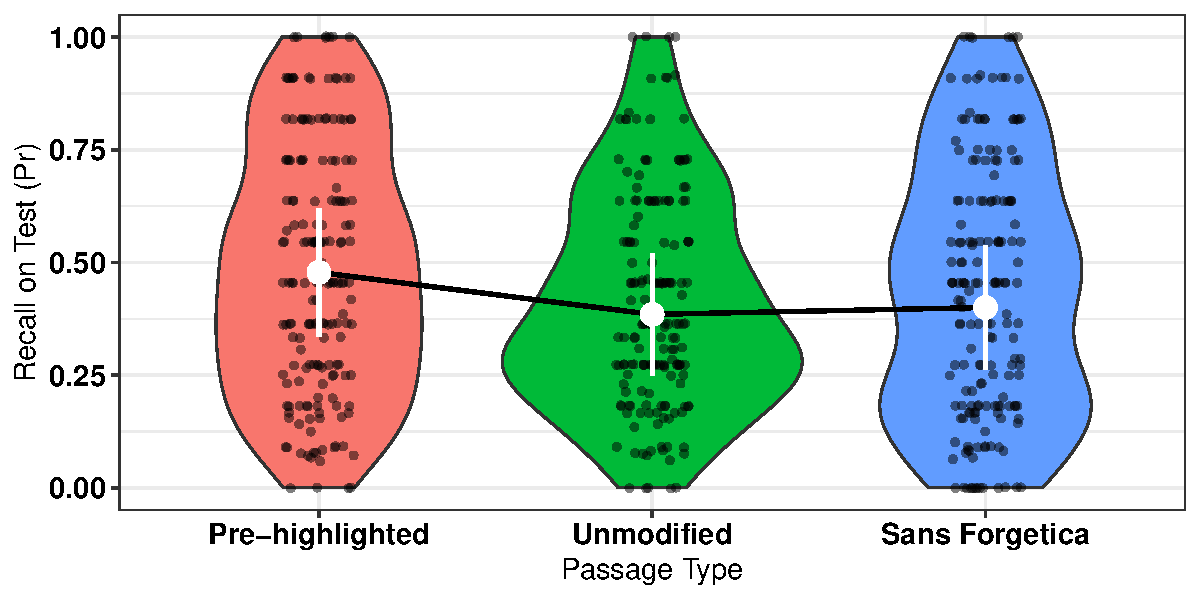
\includegraphics{SF_Paper_files/figure-latex/unnamed-chunk-3-1}

\}

\textbackslash{}caption\{Passage Cued Recall Accuracy as a function of passage type. Passage Error bars are 95\% CIs dervied from the glmer model using the effects package in R.\}\label{fig:unnamed-chunk-3}
\textbackslash{}end\{figure\}

\hypertarget{exploratory-analysis}{%
\subsection{Exploratory Analysis}\label{exploratory-analysis}}

In Experiment 2 we also asked students about their metacognitive awarness. Specifically we asked participants: \enquote{How likely is it that you will be able to recall material from the passage you just read on a scale of 0 (not likely to recall) to 100 (likely to recall) in 5 minutes?} Initial analyses suggest that the normal passage was given higher JOLs (\emph{M} = 57.4, \emph{SE} = 1.97) than the pre-highlighted passage (\emph{M} = 50.3, \emph{SE} = 1.97), t(525) = -7.08, \emph{p} = .023. There were no reliable differences between the pre-highlighted passage and Sans Forgetica (\emph{M} = 53.8, \emph{SE} = 1.97), \emph{t}(525) = -3.52, \emph{p} = .415 or between the passage in Sans Forgetica and the passage presneted normally, \emph{t}(525) = 3.56, \emph{p} = .406.

\begin{tabular}{l|r|r|r|r|r}
\hline
contrast & estimate & SE & df & t.ratio & p.value\\
\hline
Highlight - Normal & -7.079546 & 2.7792 & 525 & -2.547332 & 0.0299152\\
\hline
Highlight - Passage & -3.517046 & 2.7792 & 525 & -1.265488 & 0.4153929\\
\hline
Normal - Passage & 3.562500 & 2.7792 & 525 & 1.281844 & 0.4060534\\
\hline
\end{tabular}

\begin{figure}

{\centering 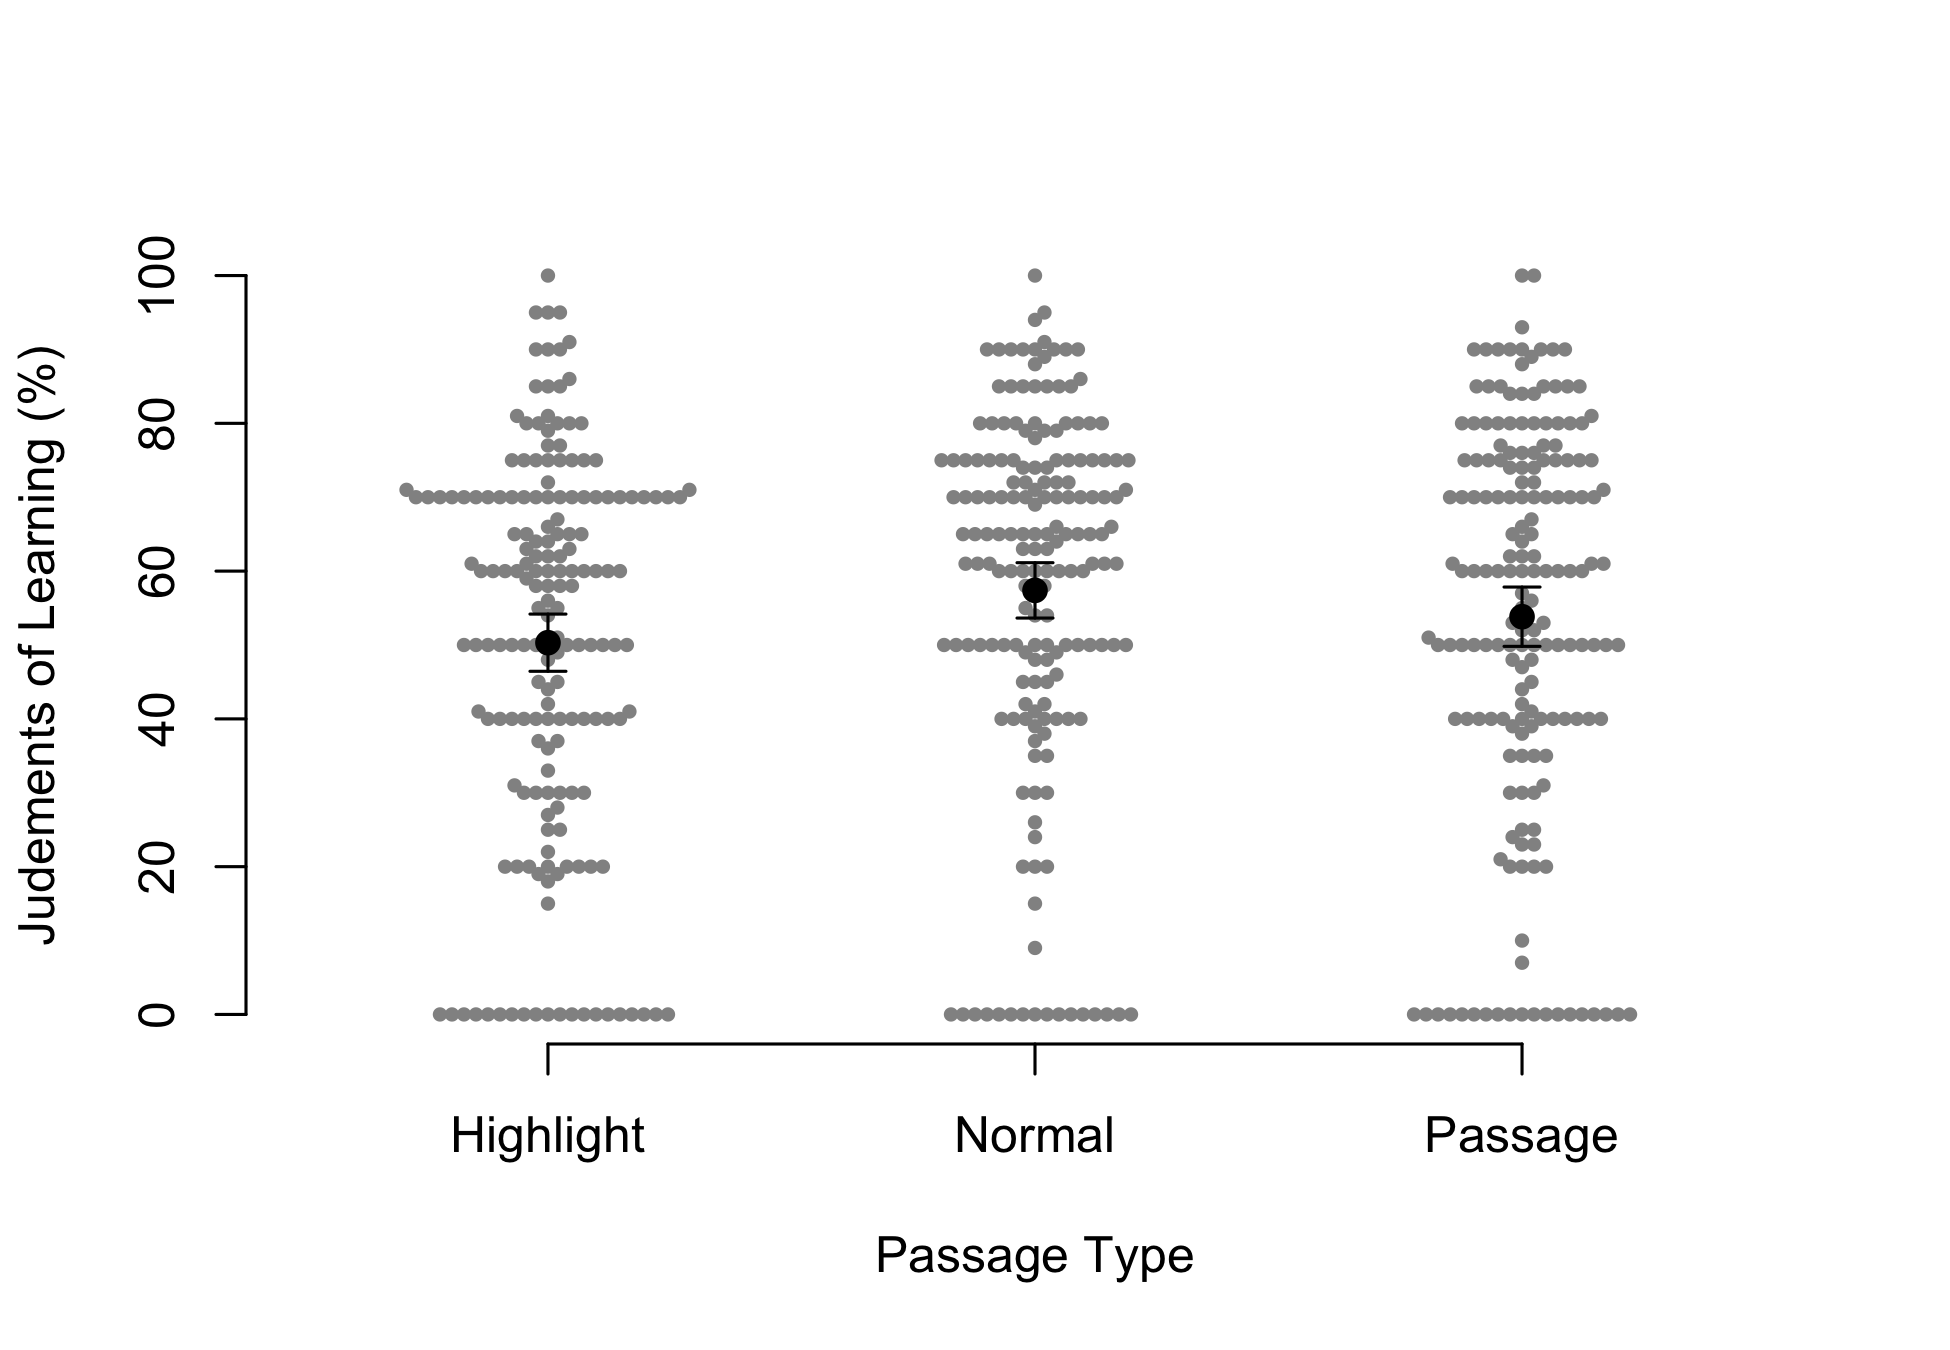
\includegraphics{SF_Paper_files/figure-latex/unnamed-chunk-4-1} 

}

\caption{Judgements of learning as a function of passage type.}\label{fig:unnamed-chunk-4}
\end{figure}

\begin{table}[tbp]

\begin{center}
\begin{threeparttable}

\caption{\label{tab:unnamed-chunk-4}}

\begin{tabular}{llllll}
\toprule
contrast & \multicolumn{1}{c}{estimate} & \multicolumn{1}{c}{SE} & \multicolumn{1}{c}{df} & \multicolumn{1}{c}{t.ratio} & \multicolumn{1}{c}{p.value}\\
\midrule
Highlight - Normal & -7.08 & 2.78 & 525.00 & -2.55 & 0.03\\
Highlight - Passage & -3.52 & 2.78 & 525.00 & -1.27 & 0.42\\
Normal - Passage & 3.56 & 2.78 & 525.00 & 1.28 & 0.41\\
\bottomrule
\end{tabular}

\end{threeparttable}
\end{center}

\end{table}

Words presented in Sans Forgetica did not lead to better recall than words left unmodifed or pre-highlighted. We did, however, observe better memory for pre-highlighted information compared to words presented unmodifed or in a Sans Forgetica font.

Examining metamemory judgments, we showed that a passage in Sans Forgetica does not produce lower judgements of learning compared to an unmodified or pre-highlighted font. Interestingly, individuals gave lower JOLs to prehighlighted information compared to materials presented in a normal font. One potential reason for pre-highlighted information recieving lower JOLs than the normal passage is that pre-highlighted information served to focus participants attention specific parts of the passage. Given the question, pariticpants might have thought this would hinder them if tested over the passage as a whole.

Taken together, these results suggests that Sans Forgetica might not be a desirable difficulty.

\hypertarget{discussion}{%
\section{Discussion}\label{discussion}}

While it has been reported that Sans Forgetica font can enhance performacne (Eskenazi \& Nix, 2020), we report results from two high-powered experiments arguing against this claim. Specifically, we demonstrated that Sans Forgetica does not enhance recall for cue-target pairs (Experiment 1) or words embeded in sentences from a passage (Experiment 2). This adds to the increasing litearture showing that perceptual disfluency has very little impact on actual memory performance (e.g., Magreehan et al. (2016); Rhodes and Castel (2008); Rhodes and Castel (2009); Rummer et al. (2016); Xie et al. (2018); Yue et al. (n.d.)), While Sans Forgetica did not produce a memory benefit, we did observe a memory advantage for items that had to be generated (Experiment 1) and that were pre-highlighted, thereby replciating previous results ().
\#\# Limitations

\hypertarget{transfer-appropriate-processing}{%
\subsubsection{Transfer-appropriate processing}\label{transfer-appropriate-processing}}

In both experiments we looked at cued recall. A recent transfer-appropriate processing (TAP) framework has contextualized when difficulties are desirable and when they are not (McDaniel \& Butler, 2011). Its essence emphasizes the qualitative mismatch of the evoked encoding processes of the applied difficulty (and by the material) with respect to the required retrieval processes of the memory test. Thus, one important aspect postulated by this framework denotes the specific encoding processes stimulated by the type of difficulty applied. For example, generating incomplete word-fragments within a text intensifies the processing of the word cue and the word surroundings that help to identify the word, thus enhancing proposition-specific encoding. In contrast, creating sentence coherency in a text with randomized sentences intensifies the processing of the relationships of information in the text, thus enhancing relational encoding (McDaniel, Hines, Waddill, \& Einstein, 1994). Consequently, the generation-task, which required word-generation, led to improved verbatim recall, but it was not desirable for relational test questions (and vice versa). These differently evoked encoding processes (proposition-specific versus relational) by the generation task predicted different memory effects. It is thus possible that the Sans Forgetica effect arises only under certain memory paradigms (e.g., free recall or recognition). It is hard to test this however, as the mechanisms that give rise to the effect are unclear and currently there is not strong evidence that the Sans Forgetica effect is reliable. Furture research should explore different testing conditions.

\hypertarget{processing-difficulty}{%
\subsubsection{Processing Difficulty}\label{processing-difficulty}}

One critism put forth when examianing perceptual disfluency is that studies do not objectively test (e.g., by using RTs) that stimuli are in fact perceptually disfluent {[}see Geller et al. (2018)). Given that the two experiments conatined herein were presented on-line using the Qualtircs platform, it was difficult to test this assumption. However, recently, a eye-tracking study by (Eskenazi \& Nix, 2020) provided evidence that Sans Forgetica is perceptually disfluent. In their study, as better spellers had longer gaze durations and spent more total time on words presented in Sans Forgetica than poor spellers. This suggests that Sans Forgetica is perceptually disfluent as long as you are a good speller.

\hypertarget{conclusion}{%
\section{Conclusion}\label{conclusion}}

The two experiments herein present evidence against claims put forth by its creators and the media {[}also see Eskenazi and Nix (2020)). We concede that our conclusions of no effect might be a bit premature. It is possible that there is an effect of Sans Forgetica, but the effect size might be smaller than we could detect acorss our two studies. We powered our studies to detect a medium-sized effect. Further, as noted by (Eskenazi \& Nix, 2020) and others {[}Geller2018; Geller2019{]} there are important moderating factors of the disfluency effect that should be considered. Once more research is published, a meta-analysis can be conducted to determine the effect size and any modertaing factors of the Sans Forgetica effect. Reagardless, it is our conclusion that Sans Forgetica lives up its name. Students looking to remmeber more and forget less should use other \enquote{power tools} shown to enhance learning.

\newpage

\hypertarget{references}{%
\section{References}\label{references}}

\begin{verbatim}
## Warning in readLines(file): incomplete final line found on 'ref.bib'
\end{verbatim}

\begingroup
\setlength{\parindent}{-0.5in}
\setlength{\leftskip}{0.5in}

\hypertarget{refs}{}
\leavevmode\hypertarget{ref-Bates2015}{}%
Bates, D., Mächler, M., Bolker, B., \& Walker, S. (2015). Fitting linear mixed-effects models using lme4. \emph{Journal of Statistical Software}, \emph{67}(1), 1--48. \url{https://doi.org/10.18637/jss.v067.i01}

\leavevmode\hypertarget{ref-Bertsch2007}{}%
Bertsch, S., Pesta, B. J., Wiscott, R., \& McDaniel, M. A. (2007). The generation effect: A meta-analytic review. \emph{Memory and Cognition}, \emph{35}(2), 201--210. \url{https://doi.org/10.3758/BF03193441}

\leavevmode\hypertarget{ref-Bjork2011}{}%
Bjork, E. L., \& Bjork, R. A. (2011). Making things hard on yourself, but in a good way: Creating desirable difficulties to enhance learning. In \emph{Psychology and the real world: Essays illustrating fundamental contributions to society.} (pp. 56--64). New York, NY, US: Worth Publishers.

\leavevmode\hypertarget{ref-Bjork2016}{}%
Bjork, R. A., \& Yue, C. L. (2016). Commentary: Is disfluency desirable? Springer New York LLC. \url{https://doi.org/10.1007/s11409-016-9156-8}

\leavevmode\hypertarget{ref-Buchanan2019}{}%
Buchanan, E. M., De Deyne, S., \& Montefinese, M. (2019). A practical primer on processing semantic property norm data. \emph{Cognitive Processing}. \url{https://doi.org/10.1007/s10339-019-00939-6}

\leavevmode\hypertarget{ref-Burkner2018}{}%
Bürkner, P.-C. (2018). Advanced Bayesian multilevel modeling with the R package brms. \emph{The R Journal}, \emph{10}(1), 395--411. \url{https://doi.org/10.32614/RJ-2018-017}

\leavevmode\hypertarget{ref-Carpenter2016}{}%
Carpenter, S. K. (2016). Spacing effects on learning and memory. In \emph{The curated reference collection in neuroscience and biobehavioral psychology} (pp. 465--485). Elsevier Science Ltd. \url{https://doi.org/10.1016/B978-0-12-809324-5.21054-7}

\leavevmode\hypertarget{ref-Carpenter2006}{}%
Carpenter, S. K., Pashler, H., \& Vul, E. (2006). What types of learning are enhanced by a cued recall test? \emph{Psychonomic Bulletin and Review}, \emph{13}(5), 826--830. \url{https://doi.org/10.3758/BF03194004}

\leavevmode\hypertarget{ref-Diemand-Yauman2011}{}%
Diemand-Yauman, C., Oppenheimer, D. M., \& Vaughan, E. B. (2011). Fortune favors the: Effects of disfluency on educational outcomes. \emph{Cognition}, \emph{118}(1), 111--115. \url{https://doi.org/10.1016/j.cognition.2010.09.012}

\leavevmode\hypertarget{ref-Earp2018}{}%
Earp, J. (2018). Q\&A: Designing a font to help students remember key information.

\leavevmode\hypertarget{ref-Eskenazi2020}{}%
Eskenazi, M. A., \& Nix, B. (2020). Individual Differences in the Desirable Difficulty Effect During Lexical Acquisition. \emph{Journal of Experimental Psychology: Learning Memory and Cognition}. \url{https://doi.org/10.1037/xlm0000809}

\leavevmode\hypertarget{ref-Fowler1974}{}%
Fowler, R. L., \& Barker, A. S. (1974). Effectiveness of highlighting for retention of text material. \emph{Journal of Applied Psychology}, \emph{59}(3), 358--364. \url{https://doi.org/10.1037/h0036750}

\leavevmode\hypertarget{ref-French2013}{}%
French, M. M., Blood, A., Bright, N. D., Futak, D., Grohmann, M. J., Hasthorpe, A., \ldots{} Tabor, J. (2013). Changing fonts in education: How the benefits vary with ability and dyslexia. \emph{Journal of Educational Research}, \emph{106}(4), 301--304. \url{https://doi.org/10.1080/00220671.2012.736430}

\leavevmode\hypertarget{ref-Geller2018}{}%
Geller, J., Still, M. L., Dark, V. J., \& Carpenter, S. K. (2018). Would disfluency by any other name still be disfluent? Examining the disfluency effect with cursive handwriting. \emph{Memory and Cognition}, \emph{46}(7), 1109--1126. \url{https://doi.org/10.3758/s13421-018-0824-6}

\leavevmode\hypertarget{ref-Jeff1961}{}%
Jeffreys, H. (1961) Theory of Probability. 3rd Edition, Clarendon Press, Oxford. - References - Scientific Research Publishing. (n.d.). Retrieved from \url{https://www.scirp.org/(S(351jmbntvnsjt1aadkposzje))/reference/ReferencesPapers.aspx?ReferenceID=1737428}

\leavevmode\hypertarget{ref-Kornell2016}{}%
Kornell, N., \& Vaughn, K. E. (2016). How Retrieval Attempts Affect Learning: A Review and Synthesis. \emph{Psychology of Learning and Motivation - Advances in Research and Theory}, \emph{65}, 183--215. \url{https://doi.org/10.1016/bs.plm.2016.03.003}

\leavevmode\hypertarget{ref-Lakens2014}{}%
Lakens, D., \& Evers, E. R. K. (2014). Sailing From the Seas of Chaos Into the Corridor of Stability: Practical Recommendations to Increase the Informational Value of Studies. \emph{Perspectives on Psychological Science : A Journal of the Association for Psychological Science}, \emph{9}(3), 278--292. \url{https://doi.org/10.1177/1745691614528520}

\leavevmode\hypertarget{ref-Magreehan2016}{}%
Magreehan, D. A., Serra, M. J., Schwartz, N. H., \& Narciss, S. (2016). Further boundary conditions for the effects of perceptual disfluency on judgments of learning. \emph{Metacognition and Learning}, \emph{11}(1), 35--56. \url{https://doi.org/10.1007/s11409-015-9147-1}

\leavevmode\hypertarget{ref-McDaniel2011}{}%
McDaniel, M. A., \& Butler, A. C. (2011). A contextual framework for understanding when difficulties are desirable. In \emph{Successful remembering and successful forgetting: A festschrift in honor of robert a. Bjork.} (pp. 175--198). New York, NY, US: Psychology Press.

\leavevmode\hypertarget{ref-McDaniel1994}{}%
McDaniel, M. A., Hines, R. J., Waddill, P. J., \& Einstein, G. O. (1994). What Makes Folk Tales Unique: Content Familiarity, Causal Structure, Scripts, or Superstructures? \emph{Journal of Experimental Psychology: Learning, Memory, and Cognition}, \emph{20}(1), 169--184. \url{https://doi.org/10.1037/0278-7393.20.1.169}

\leavevmode\hypertarget{ref-Mulligan1996}{}%
Mulligan, N. W. (1996). The effects of perceptual interference at encoding on implicit memory, explicit memory, and memory for source. \emph{Journal of Experimental Psychology: Learning Memory and Cognition}, \emph{22}(5), 1067--1087. \url{https://doi.org/10.1037/0278-7393.22.5.1067}

\leavevmode\hypertarget{ref-Nelson2004}{}%
Nelson, D. L., McEvoy, C. L., \& Schreiber, T. A. (2004). The University of South Florida free association, rhyme, and word fragment norms. Psychonomic Society Inc. \url{https://doi.org/10.3758/BF03195588}

\leavevmode\hypertarget{ref-Ooms2018}{}%
Ooms, J. (2018). \emph{Hunspell: High-performance stemmer, tokenizer, and spell checker}. Retrieved from \url{https://CRAN.R-project.org/package=hunspell}

\leavevmode\hypertarget{ref-Rhodes2008}{}%
Rhodes, M. G., \& Castel, A. D. (2008). Memory Predictions Are Influenced by Perceptual Information: Evidence for Metacognitive Illusions. \emph{Journal of Experimental Psychology: General}, \emph{137}(4), 615--625. \url{https://doi.org/10.1037/a0013684}

\leavevmode\hypertarget{ref-Rhodes2009}{}%
Rhodes, M. G., \& Castel, A. D. (2009). Metacognitive illusions for auditory information: Effects on monitoring and control. \emph{Psychonomic Bulletin and Review}, \emph{16}(3), 550--554. \url{https://doi.org/10.3758/PBR.16.3.550}

\leavevmode\hypertarget{ref-Rosner2015}{}%
Rosner, T. M., Davis, H., \& Milliken, B. (2015). Perceptual blurring and recognition memory: A desirable difficulty effect revealed. \emph{Acta Psychologica}, \emph{160}, 11--22. \url{https://doi.org/10.1016/j.actpsy.2015.06.006}

\leavevmode\hypertarget{ref-Rummer2016}{}%
Rummer, R., Schweppe, J., \& Schwede, A. (2016). Fortune is fickle: null-effects of disfluency on learning outcomes. \emph{Metacognition and Learning}, \emph{11}(1), 57--70. \url{https://doi.org/10.1007/s11409-015-9151-5}

\leavevmode\hypertarget{ref-Silvers1997}{}%
Silvers, V. L., \& Kreiner, D. S. (1997). The effects of pre-existing inappropriate highlighting onreading comprehension. \emph{Reading Research and Instruction}, \emph{36}(3), 217--223. \url{https://doi.org/10.1080/19388079709558240}

\leavevmode\hypertarget{ref-Sungkhasettee2011}{}%
Sungkhasettee, V. W., Friedman, M. C., \& Castel, A. D. (2011). Memory and metamemory for inverted words: Illusions of competency and desirable difficulties. \emph{Psychonomic Bulletin and Review}, \emph{18}(5), 973--978. \url{https://doi.org/10.3758/s13423-011-0114-9}

\leavevmode\hypertarget{ref-Wickham2016}{}%
Wickham, H. (2016). \emph{Ggplot2: Elegant graphics for data analysis}. Springer-Verlag New York. Retrieved from \url{https://ggplot2.tidyverse.org}

\leavevmode\hypertarget{ref-Xie2018}{}%
Xie, H., Zhou, Z., \& Liu, Q. (2018). Null Effects of Perceptual Disfluency on Learning Outcomes in a Text-Based Educational Context: a Meta-analysis. \emph{Educational Psychology Review}, \emph{30}(3), 745--771. \url{https://doi.org/10.1007/s10648-018-9442-x}

\leavevmode\hypertarget{ref-Yue}{}%
Yue, C. L., Storm, B. C., Kornell, N., Ligon Bjork, E., Yue, C. L., Storm, B. C., \ldots{} Bjork, E. L. (n.d.). Highlighting and Its Relation to Distributed Study and Students' Metacognitive Beliefs. \url{https://doi.org/10.1007/s10648-014-9277-z}

\endgroup

\clearpage
\theendnotes

\end{document}
